\documentclass[border=4pt]{standalone}
% Preámbulo común de las figuras. Cada figura es un documento standalone
% que se compila a SVG con scripts/build_figures.sh
\usepackage[utf8]{inputenc}
\usepackage{amsmath}
\usepackage{tikz}
\usepackage[american, siunitx]{circuitikz}
\usetikzlibrary{arrows.meta,calc,decorations.pathmorphing,patterns}
\tikzset{
  >={Stealth[length=2.2mm]},
  eje/.style={->, thin},
  hilo/.style={thick},
}
% Paleta común: tonos medios legibles sobre fondo claro
\definecolor{azul}{RGB}{31,94,168}
\definecolor{rojo}{RGB}{192,57,43}
\definecolor{verde}{RGB}{39,128,73}
\definecolor{naranja}{RGB}{211,120,30}
\definecolor{morado}{RGB}{125,60,152}

\begin{document}
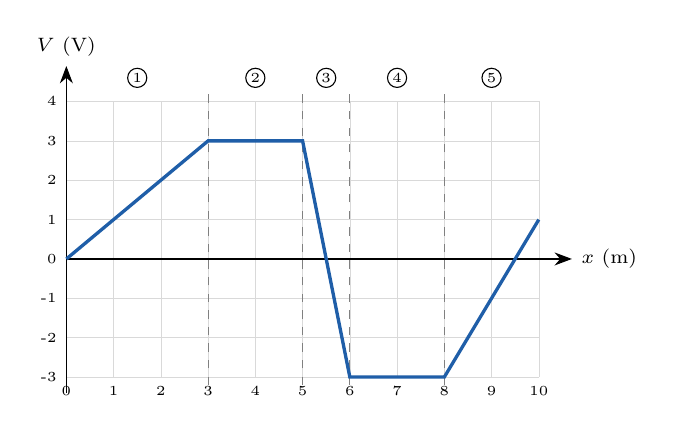
\begin{tikzpicture}[xscale=0.6, yscale=0.5]
  \draw[gray!30, very thin] (0,-3) grid (10,4);
  \draw[->] (0,0) -- (10.7,0) node[right, font=\scriptsize]{$x$ (m)};
  \draw[->] (0,-3.4) -- (0,4.9) node[above, font=\scriptsize]{$V$ (V)};
  \foreach \x in {3,5,6,8} \draw[dashed, gray] (\x,-3.2) -- (\x,4.3);
  \foreach \x in {0,1,...,10} \node[below, font=\tiny] at (\x,-3) {\x};
  \foreach \y in {-3,-2,...,4} \node[left, font=\tiny] at (0,\y) {\y};
  \draw[very thick, azul] (0,0) -- (3,3) -- (5,3) -- (6,-3) -- (8,-3) -- (10,1);
  \foreach \x/\n in {1.5/1,4/2,5.5/3,7/4,9/5} \node[circle, draw, inner sep=0.8pt, font=\tiny] at (\x,4.6) {\n};
\end{tikzpicture}
\end{document}
